\section{Exoplanetary Context}\label{sec:ch1_context}

    Over the last three decades, the plethora of exoplanetary system detections has revolutionized the way we understand how planetary systems form and evolve. Since the discovery of the first extrasolar planets (exoplanet) around a main-sequence star, (HD~114762~b and 51~Pegasi~b \textbf{reference}), a revolution has occurred in our understanding of planetary formation and evolution. We have seen exoplanets of a variety of flavors; gas giants at fractions of an astronomical unit (AU) from their star, binary planetary systems, compact multi-planet systems. Giant planets are found with eccentricities ranging from 0--0.9, with sometimes large mutual inclinations. And roughly 50\% of solar type stars have a chance of hosting a compact multi-planet system with periods shorter than a year \textbf{see Review by Winn \& Fabrycky 2015}. 
    
    In contrast, in our Solar System, the planets follow nearly circular, low inclination orbits at distances that separate terrestrial and gas giants (see \S~\textbf{Section on Solar System}). Of course there are a few exoplanetary systems that may seem architecturally similar to our own. The HR~8799 multi-planet system is the perfect example, where its four directly imaged giant planets are at the same distance from the HR8799 star as our Jovian planets are, scaled to the Luminosity of our Sun \textbf{Reference and/or image}. 
    
    
    However, a number of questions arise if we try to place the origin of our Solar System in context to the diversity of exoplanetary systems:  differences between the Solar System and what we have observed around other stars leads to a number of questions. Can we truly understand the diversity of planetary systems? Is the existence of another habitable planet likely? If so, how can we identify such systems?
    %===================================================================
    %                DIVERSITY OF EXOPLANETS
    %===================================================================
    \begin{figure}
    \centering
    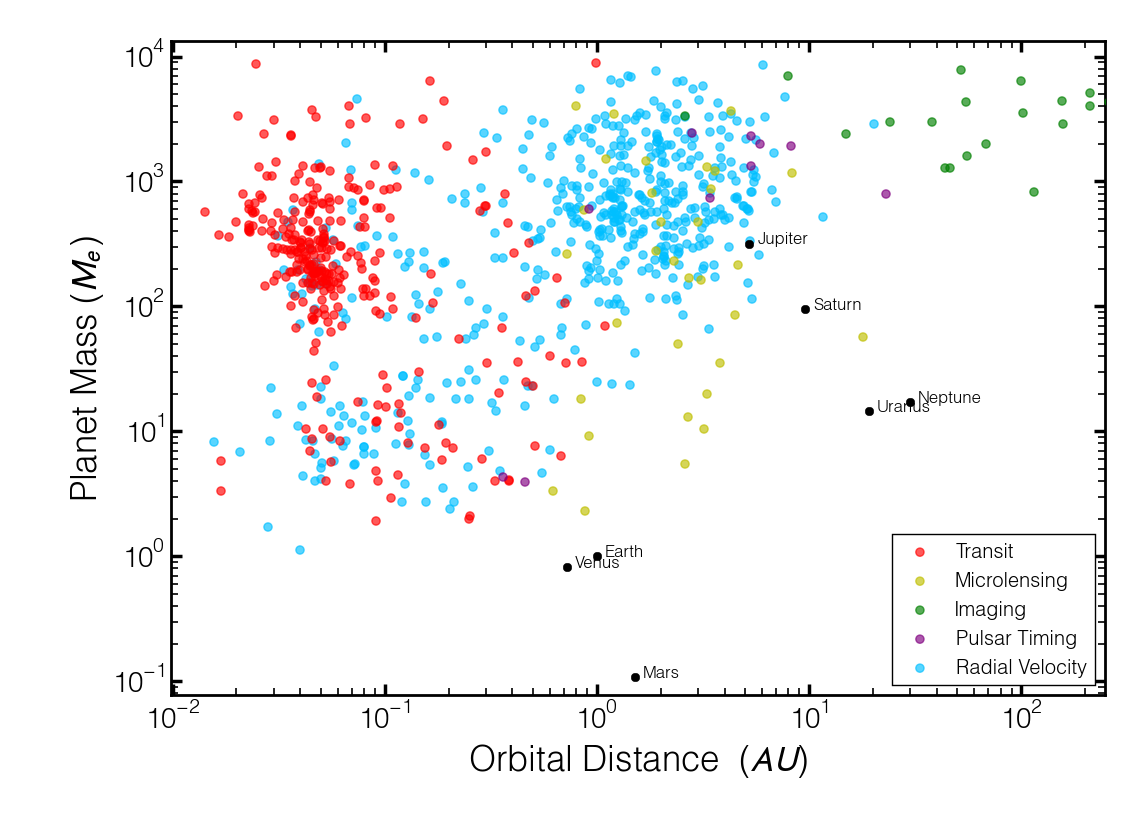
\includegraphics[scale=0.6]{Ch1/exoplanet_detections_june2015} 
    \caption[Exoplanet Statistics]{Not representative of all plaents -- those that don't have distances are not plotted. Mix of msini and m listed.}
    \label{fig:known_exoplanets}
    \end{figure}
    %===================================================================
    
    Since the template of our Solar System is a requirement to address the above questions, it is fitting to investigate the Solar System in greater detail. One aspect of our Solar System that can be used to place its origin and evolution in context is via the circumsolar debris disk. Given that our own debris disk is created from the interplay between the planets and the minor bodies, studying exo-debris disks can inform us of potentially undiscovered planetary systems, as well as help place our own Solar System in context. Thus, the next question to ask is whether nature can mimic a similar disk architecture such as ours and how we our system fits into the backdrop of the multitude of planetary system detections. 
    
    This thesis takes a step toward answering such profound questions by identifying additional systems which have previously been overlooked and may hold a wealth of information in terms of...
    
    
    
\section{The Solar System's Debris Disk}\label{sec:ch1_ssdisk}

     \subsection{Current Configuration}
    
    Since I will be discussing debris disk detections motivated by the need to place our Solar System in context, it only makes sense to discuss in some detail our own Solar System's planetary system. The eight planets in the Solar System are follow a rather orderly configuration. The orbits are close to circular ($<0.21$), and are closely inclined to the invariable plane, ranging from $0.33^{\circ}$--$2.19^{\circ}$. The latter fact applies to all the planets except for Mercury, which has an inclination of $6.3^{\circ}$. The four rocky planets are located interior to 1.7~AU, while the four gas giant planets are located beyond the snow-line -- the point in relation to the Sun beyond which volatile molecules (e.g.,$H_20, CH_4$) condense -- all the way out to 30~AU. 
    
    %===================================================================
    %                  THE SOLAR SYSTEM DIAGRAM
    %===================================================================
    %\begin{figure}
    %\centering
    %\includegraphics[scale=0.6]{Ch1/???} 
    %\caption{Caption}
    %\label{fig:solar_system}
    %\end{figure}
    %===================================================================
    
    
    
    The inner and outer planets are also segregated by a physical barrier known as the Asteroid belt. Located between the orbit of Mars and Jupiter, the Asteroid belt spans a width of XX~AU and is composed of over a million kilometer-sized \textbf{check fact} objects that can be metallic, stony or even carbon rich in composition. In recent studies, some asteroids, such as $24 Themis$, have been found to be covered by an water-ice mantle \citep{Campins2010}. It has been estimated that the mass of the Asteroid belt is XX Mearths, a value that was much larger in the early Solar System (see \S~\ref{sec:solar_system}. Beyond the orbit of Neptune lies a large reservoir or minor planets composed of icy, volatile, cometary material with sizes greater than XX. These minor bodies, distributed in a thin belt the width of XX~AU, are known as the Edge-Worth Kuiper Belt (EKB). \textbf{Maybe give a reference for a larger review?}.
    
    %===================================================================
    %               THE Zodiacal Dust 
    %===================================================================
    \begin{figure}
    \centering
    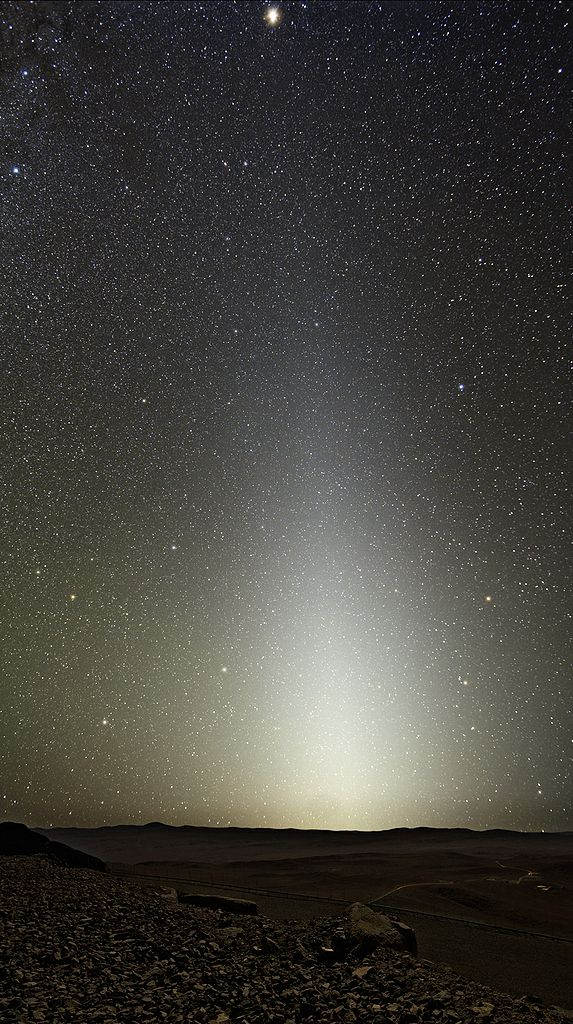
\includegraphics[scale=0.95]{Ch1/Zodiacal_Light_Paranal} 
    \caption[Zodiacal Light On Earth]{Zodiacal Light by ESO. Reference to ZD picture http://www.eso.org/public/unitedkingdom/images/zodiacal-light/}
    \label{fig:ZD_ESO}
    \end{figure}
    %===================================================================
    
    
    
    In addition to the rings of large rocky bodies, a disk composed of 10--100$\mu m$ sized cometary and silicate grains inhabits the Solar System. This disk, known as the Zodiacal Cloud, has been seen in scattered light observations (Hahn+2002), thermal emission from the Planck \citep{Maris2006}, COBE \citep{Kelsall1998}, and the \textit{Infrared Astronomical Satellite} (Sykes 1990) missions, as well as from spacecraft impact experiments. From the ground, the Zodiacal Cloud can be seen only on the darkest of skies, as a faint glow along the ecliptic (see Figure~\textbf{Figure of ZD}). The inner Zodiacal Cloud extends from the orbit of Venus all the way out to Jupiter. From most recent studies, namely \citet{Nesvorny2010}, the small particles which comprise the disk are thought to be mainly created from the grinding down of mm--cm sized grains, which themselves are ejected by spontaneous disruption from Jupiter Family Comets (JFC) as they approach the large tidal forces of Jupiter's gravity. The overall mass of the inner Zodiacal Cloud has been estimated to be $\sim1-2\times10^{19}$~g. To place this number into perspective, the bolometric Luminosity of the disk compared to that of the Sun is $L_{ZODY}/L_\odot \sim 2\times10^{-7}$. 


    
    \subsection{Dynamical Evolution Of Our Planetary System}\label{sec:solar_system}
    
    Beyond just learning about the structure of the present-day Solar System, it is important to understand how the Solar System evolved into what we see now. This is for many reasons, but mainly because it is the only system where we know life exists. Although it is impossible to detail the entire history of the Solar System's evolution, it is important to understand that the current architecture of the Solar System would not be possible without the combined evolution of the planets as well as the remnant asteroidal and cometary disks. 
    
    It is generally accepted that the planets formed within the first 100 Myr (upper limit based on the final accretion to create Earth \citep{Allegre2008}), after the Sun reached its place on the main-sequence. During this time, it is thought that the planets were in a more compact configuration, within 15~AU \citep{Batygin2010}. Roughly 4.0--3.7 Gyr ago, scattering of the planetismal populations that lay outside the orbit of Neptune at 15~AU resulted in angular momentum exchange between the Gas Giants and the disk. This led to a period of instability, in which Jupiter and Saturn's orbits diverged, eventually crossing their mutal 1:2 mean motion resonance. From this, Jupiter migrated inward by $<0.5$~AU \citep{Morbidelli2010}, and pushed Saturn, Uranus and Neptune further out into the Solar System \citep{Tsiganis2005}. 
    
    This migration led to a period known as the Late Heavy Bombardment (LHB). During this time, Jupiter's short migration would have depleted the Asteroid belt by a factor or 10, and 97\% of the EKB was probably removed as a result of Neptune's outward migration. The scattered comets and asteroids during this period are most likely responsible for the Lunar craters \citep{Gomes2005}. However, it is also thought that the majority of Earth's water supply was transported during the LHB either from the EKB or from water rich asteroids. In addition, the depletion of the Asteroid belt by Jupiter has implications for the emergence of life on Earth, as a massive Asteroid belt today would imply a higher frequency of Terrestrial impacts. 
    
    \textbf{Some last sentence/paragraph on just one example and that w/o the disk, perhaps the planets would not be where they are, and Earth may not have the necessary resources to allow life to flourish. Also add in a line about how we would like to witness this type of evolution around other stars to place the SS in context.}
    
    %LHB lasted between 10 and 150 Myr
    %various resonance structures now in SS (Jupiter and AB, Neptune and KB)
    
      % Due to the gravitational influence of Jupiter, a number of (resonances)


%INSERT FIGURE OF ZD BRIGHTNESS DISTRIBUTION FROM NESVORNY 2010 (Fig 17.


\section{Circumstellar Disk Evolution}
    
    To understand something something in context of solar system, 
    The majority of disks are detected from the excess radiation in the infrared at levels greater than expected from the stellar photosphere (i.e., infrared excess), which arises from the heating of gas and dust in in the circumstellar environment. A detailed discussion of this will be in \S~\textbf{section on debris disk detections}


    \subsection{Protoplanetary Disk Evolution}
    
    The paradigm of planet formation begins with a nascent protoplanetary disk (PPD), with primordial gas and dust that remains post-star formation, and which is then used to build the planets that we have detected. The primordial material forms into a circumstellar disk, as a consequence of angular momentum conservation. and is heavily sensitive to the angular rotation of the central star ($\Omega^2$) and even more sensitive to the infall time of the primordial material ($t_{infall}^3$) \citep{Terebey1984}. It is well accepted that 90-99\% of a PPD, is composed of gas, with the rest in the form of mm to micron sized dust grains. The bulk of the gas is comprised of neutral $H_2$, and mid-IR rotational lines have been observed from hot ($>600$~K) $H_2$ from the ground in the AB~Aur system \citep{Bitner2007}. Typically, however, tracers such as $CO$, and $HCN$ line emissions are observed at sub-mm wavelengths to detect the gas in PPDs (e.g. for stars in young associations such as Ophiuchus \citep{Andre1994} and Taurus-Auriga \citep{Beckwith1990}). These type of observations have shown that the size of these disks can range from 10--100~AU, with masses $>0.005M_\odot$ \citep{Osterloh1995}. These dust masses are typically derived by excess fluxes at mm-wavelengths, with extrapolations of the spectral distribution by assuming an upper limit to the grain size (usually around mm sizes) and some assumed opacity values \citep{Beckwith1990}. Figure~\ref{fig:disk_masses} shows the masses of observed PPDs (ages $<10$~Myr), indicating disk masses on the order of a few hundred $M_{earth}$. 
    
    %===================================================================
    %   DISK MASSES FIG 3 WYATT 2008
    %===================================================================
    %\begin{figure}
    %\centering
    %\includegraphics[scale=0.6]{Ch1/???} 
    %\caption{Caption}
    %\label{fig:disk_masses}
    %\end{figure}
    %===================================================================
    
    Within the first $\sim$10~Myr, the majority of the primordial gas and dust has dissipated. Viscous accretion of gas and dust onto the star has been attributed to the clearing of the inner regions (a few AU) of the star, which is supported by a lack of near-IR flux (2--5$\mu m$) and the presence of forbidden line accretion signatures \citep[(e.g., O~I, S~II)][]{Hartigan1995}. Photoevaporation from the central star will also carve out the outer disk. In this process, high-energy UV and X-Ray photons can excite gas and dust molecules enough so that they are no longer bound to the system, and simply evaporate into interstellar space. The replenishment of material into the inner disk after the viscous accretion has halted, is inhibited from extreme-UV photons from the central star. The disk can also be dissipated via external sources. Usually, young stars are found in clusters with thousands of stars. A few of these will be O stars, that irradiate the surrounding environment in intense ionizing UV radiation. From this, mass loss of the disk can become expedited. 
    
    During this entire process, grain-growth becomes important, as it not only removes mass from the gas rich, but also provides the seeds for future planetary creation. Small micron sized grains will typically feel a pressure gradient, since the gas rotates at non-Keplerian speeds. From this, grains will eventually collide, increase in mass and size, and be dragged to the mid-plane of the disk, where they can further grow to form the cores of potential planets, as well as asteroids and comets. The presence of any fully formed planets within this time can start sculpting  Figure~\ref{fig:ppd_2_dd} illustrates these different processes dissipating the overall mass of the disk.
    
    %===================================================================
    %   ILLUSTRATION OF EVOLUTION OF PPD TO DEBRIS DISK
    %===================================================================
    %\begin{figure}
    %\centering
    %\includegraphics[scale=0.6]{Ch1/???} 
    %\caption{Caption}
    %\label{fig:ppd_2_dd}
    %\end{figure}
    %===================================================================
    
    It has been observed that once the inner disk ($<$5~AU) is depleted, the outer disk quickly loses the majority of its mass \citep{Williams2011}. Thus, after about 6--10 Myr, most stars have lost their inner disks, as determined from the stars near-IR excess emission \citep{Wyatt2008}. Figure~\ref{fig:ppd_near_irexcess} shows the rapid decline in disk fraction as a function of age for a number fo different young stellar clusters and associations, illustrating that the fraction of stars with near-IR excesses dwindles down to $\sim$0\%. 
    
    %===================================================================
    %   EVOLUTION OF NEAR-IR EXCESS IN PPDS WYATT2008 FIG 2
    %===================================================================
    %\begin{figure}
    %\centering
    %\includegraphics[scale=0.6]{Ch1/???} 
    %\caption{Caption}
    %\label{fig:ppd_near_irexcess}
    %\end{figure}
    %===================================================================
    
        
    \subsection{Debris Disk Evolution}\label{sec:debrisdisk_phase}
    
    What remains from the remnant PPD after the bulk of the gas has dissipated, is typically a disk composed of planetesimals and dust population (illustrated in Figure~\ref{fig:ppd_2_dd}). From studies (\textbf{e,g,Lisse	et	al.	2009, (Lisse	et	al.	2012) 	De	Vries	et	al.	(2012), Rodigas2015}) we know that the dust in a circumstellar disk can be composed of macroscopic particles, ranging in sizes from mm scales to $<100$\micron in and heterogeneously composed of various minerals: silicates, other dielectric and refractory particles as well as volatiles compounds (e.g., ice, Carbon Monoxide). We know from observations of debris disks at sub-mm wavelengths, that dust masses are orders of magnitudes lower than in the gas-rich PPD phase of the disk; typically on the order of less than an Earth mass (see Figure~\ref{fig:disk_masses}). 

    For grains larger than $\sim$ 1~mm (e.g., large grains, small planetesimals), their motions are governed by the gravitational force from the central star. 
    The low mass of these disks implies that debris disks are optically thin, meaning that the majority of the radiation that passes through the disk is seen by the observer. Thus, for smaller grains of size $s<1$~mm, stellar radiation and stellar wind play an important role in the dynamical behavior of the dust. The force exerted on a particle from radiation pressure $F_r$ counteracts the radial gravitational force. Thus the photogravitational force is written as
    
    \begin{equation}\label{eq:photograv_force}
    \left|\vec{F_{pg}}\right|= \frac{GM_\star m_g(1-\beta)}{r_d^2}
    \end{equation}
    
    \noindent where $\beta$ is the ratio of the radiation to gravitational pressure, and is inversely proportional to the stellar luminosity, grain density and size \citep{Burns1979}. In other words, smaller particles will be influenced largely by radiative forces, rather than gravitational ones. Grains for whose bulk and optical properties produce $\beta=0.5$ experience equal gravitational and radiation pressure and represent the minimum size $s$ below which grains will be ejected from that particular system (blow-out size). In the Solar System, this corresponds to sub-micron sized grains. In addition to radiation pressure, stellar wind pressure created from high velocity plasma, aids in counteracting the gravitational force dust grains feel. 
    
    In the azimuthal direction (i.e., along the motion vector of the grain), corpuscular drag from the stellar wind will remove the orbital momentum of the dust grain and cause it to spiral out of its orbit and eventually collide into the star. However, this becomes more important for grains smaller than 0.001$\mu m$. Drag from stellar radiation, or Poynting-Robertson (P-R) drag, has a larger effect on grains in contrast. The P-R effect will remove grains from a system, by decreasing their orbital momentum, and causing them to spiral into the central star. The P-R force is defined by
    
    \begin{equation}\label{eq:pr_drag}
    |\vec{F_{PR}}| = \frac{S\pi a^2 Q_{PR}r_d^2 v}{c^2},
    \end{equation}
    
    \noindent where $S$ is the stellar flux density $Q_{PR}$ is the radiation pressure coefficient and $v$ is the velocity of the grain in the direction normal to the radiation vector (i.e., orbital direction)\citep{Burns1979}. \textbf{P-R drag works by an inhomogenous momentum exchange...reword}.
    
    %===================================================================
    %   PR Drag
    %===================================================================
    \begin{figure}
    \centering
    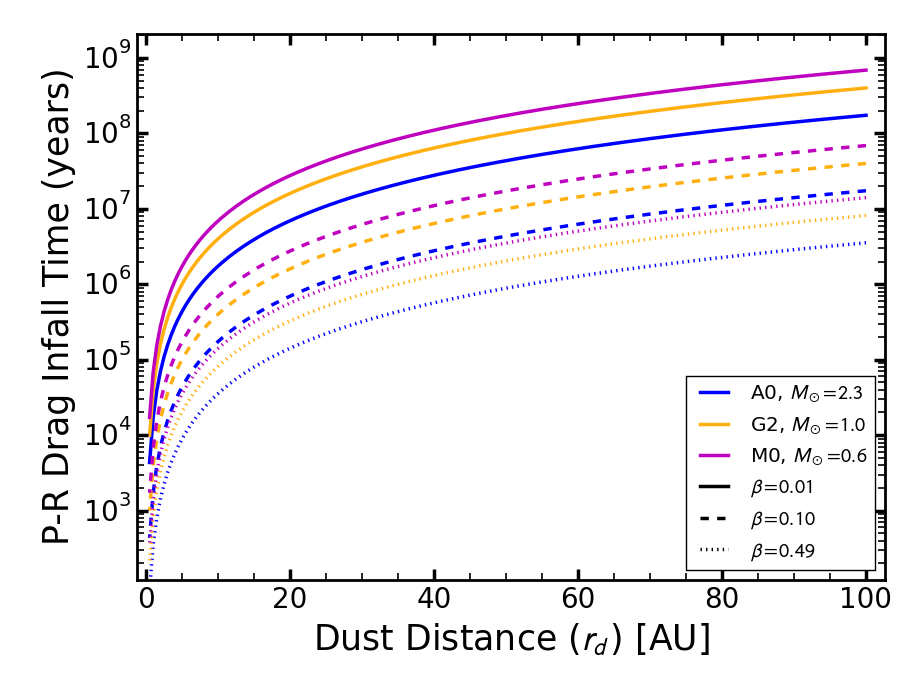
\includegraphics[scale=0.7]{Ch1/PR_Drag_time} 
    \caption{Caption}
    \label{fig:PR_Drag_time}
    \end{figure}
    %===================================================================
    
    
    
    From this we can see that grains will be removed from a system by both attractive and repellent forces. We can estimate the lifetime of a small grain under 
    
    Another important 
    
    
However, since most debris disks detected so far are too massive, they should not be considered to be heavily influenced by P-R drag \citep{Wyatt2005}. This is different, however, from saying that P-R forces have no role to play in the evolution of the disk.
    

\section{Detecting Debris Disks}\label{sec:detect_dd}

    \subsection{Dust Thermal Emission}

    Circumstellar dust immersed in the radiation field of its host star, will both scatter and absorb incoming radiation. Though most types of grains are effective scatterers in the optical and near-IR (see \textbf{\S~section on resolved imaging}), a tiny fraction of that light is absorbed and heats the dust. Grains which are smaller will heat up faster and radiate more efficiently than larger grains of the same composition and distance \citep{Krivov2010}. However, differentiating scattered versus stellar radiation becomes difficult since main-sequence stars at $T_\star>3000$~K have peak emission in the optical and near-IR ($0.4--2.5$\micron), thus increasing the contrast between scattered and stellar light. Re-emitted thermal emission is much easier to detect, since the peak emission occurs at mid ($10--30\mu m$) and far-IR ($>30\mu m$) wavelengths, regimes where the stellar photospheric emission is magnitudes fainter than the observed dust thermal emission.  
        
    Small dust grains, on the order of tens of microns, are responsible, in part, for thermal emission seen from a star in the mid- and far-IR. It is typically assumed that the grains are in thermal equilibrium with the stellar radiation field. The amount of energy a grain absorbs (mainly in the UV and optical) $E_{abs}$, is dependent on its size $a$, radial distance from the star $r_d$, the stellar luminosity $L_\star$ and the absorption efficiency $Q_{abs}(a,\lambda)$
    
    \begin{eqnarray}\label{eq:energy_absorbed}
    E_{abs} &=& \left(\frac{\pi a^2}{4\pi r_d^2}\right) \int_0^\infty L_{\lambda} Q_{abs}(a,\lambda) d\lambda \\
            &=&  \frac{a^2}{4r_d^2}L_\star \langle Q_{abs}\rangle_{UV}, 
    \end{eqnarray}
    
    \noindent while the energy emitted by the grain $E_{r}$ depends on the grain size the emitting efficiency $Q_{r}(a,\lambda)$ and is approximated by
    
    \begin{eqnarray}
    E_{r} &=& 4\pi a^2 \int_0^\infty \pi Q_{r}(a,\lambda) B(\lambda,T_d)  d\lambda \label{eq:energy_emitted1}\\
          & \approx & \left(2\pi a\right)^2 \sigma T_d^4 \langle Q_{r}\rangle_{IR}. \label{eq:energy_emitted2}
    \end{eqnarray}
            
    
    \noindent As standard practice, I've assumed an average absorption and emitting efficiency for the grain, which can be derived using Mie Theory. If we assume the grain emits as a blackbody, the expression derived in equation~\ref{eq:energy_emitted2} naturally falls into place. Conservation of energy dictates that
            
            
    \begin{equation}\label{eq:conserve_energy} 
     \frac{a^2}{4r_d^2}L_\star \langle Q_{abs}\rangle_{UV} \approx \left(2\pi a\right)^2 \sigma T_d^4 \langle Q_{r}\rangle_{IR},
    \end{equation}
            
    \noindent which leads to an approximate expression to calculate the dust temperature
    
    \begin{equation}\label{eq:tdust_full}
    T_d \approx \left(\frac{\langle Q_{abs} \rangle_{UV}}{\langle Q_{r}\rangle_{IR}} \frac{L_\star}{16\sigma \pi^2 r_d^2}\right)^{1/4}
    \end{equation}
        
    In most cases, the amount of information obtained from the dust emission is only sufficient to satisfy the simplest emission models: grains that emit as blackbodies. In the blackbody assumption, equation~\ref{eq:tdust_full} reduces to 
            
    \begin{equation}\label{eq:blackbody_temp}
            T_D = 278 \frac{\left(L_\star/L_\odot \right)^{1/4}}{\sqrt{r_D}}\enspace [K]. 
    \end{equation}
    
    \noindent assuming that $\langle Q_{abs} \rangle_{UV} \approx \langle Q_{r}\rangle_{IR}$, and scaling the stellar luminosity to the stellar luminosity $L_\odot$. In a more general sense, the grain equilibrium temperature can vary as it depends on the composition and size of the grain\citep{Drain2003}. Grains that deviate from the blackbody approxmiation will have non-zero absorption and emission efficiencies, and moderate the slope of the Wien and Rayleigh-Jeans tails of the grain emission spectrum. Around a Sun-like star, unless the dust orbits at $r_d<0.1$~AU, the grain temperatures will be $T_d \lesssim 300$~K. Following Wien's approximation, this means that the dust emission spectrum will peak in the mid- and far-IR wavelengths. Thus,astronomers will typically search for the presence of dust at IR wavelengths. 
    %    Figure~\textbf{Figure of surface plot} shows how Equation~\ref{eq:blackbody_temp} varies as a function of both stellar luminosity and stellocentric distance. In the majority of cases, grains are are heated to temperatures between 50--300~K. Temperatures above this are rarely found as these grains require close proximity to the star, and are unstable in their orbit. Smaller grains are inefficient emitters and will tend to be hotter than blackbody grains at the same distance from the star. \textbf{maybe put some equation here for it}.
    

    \subsection{Identifying Debris Disks}

    The majority of disk systems are identified through unresolved emission via photometric or spectroscopic imaging techniques. Since the dust is thermally emitting, the flux measured from a star is composed of both the stellar and dust emission. To characterize the dust emission, astronomers must accurately measure the amount of flux contributed from the star. Usually, the stellar photospheric emission in the IR, where the dust emission peaks, is estimated by extrapolating the stellar photospheric emission into the IR, from fits to stellar models using photometric or spectroscopic data in the optical and near-IR. In this regime, the luminosity of the star is large enough to overwhelm any dust emission. Figure \textbf{SED figure with model fit} shows this fit along with the blah blha blah. \textbf{Description of finding excesses using color instead of photospheric fits.} The excess flux, which is the measured flux subtracted from the estimated stellar photospheric flux, represents the thermal emission from any circumstellar dust
        
        The amount of excess flux at a particular wavelength can be characterized by the measured flux to the photospheric emission, or the relative flux of the excess
        
        \begin{equation}\label{eq:rel_excess}
        R_\lambda = F_\lambda / F_{\star,\lambda}.
        \end{equation}
        
        \noindent The fractional luminosity of the IR excess $f_d$ characterizes the total emission spectrum, or bolemtric luminosity, of the dust with respect to the bolometric stellar luminosity
        
        \begin{equation}\label{eq:rel_excess}
        f_d = L_{IR}/L_{\star}.
        \end{equation}
        
        \noindent The fractional luminosity can provide a rough estimate of the total amount of dust in the system by assuming a homogeneous composition of dust throughout the disk \citep{Wyatt2008}. A better estimate can be derived from the flux of the excess and once emissivity properties of the dust are known \citep{Beckwith2000}. As stated in \S~\ref{sec:dd_v_pd}, a debris disk, unlike a primordial disk, has a smaller gas to dust ratio. Since these disks are primarily optically thin, their IR excesses, and consequently their fractional luminosities, are smaller. A debris disk is typically characterized by \textbf{$f_d<$something}.
    
    \subsection{Is It A Debris or Protoplanetary Disk?}
    
    As illustrated in Figure~\ref{fig:ppd_2_dd}, the transition out of a PPD, broadly speaking, occurs with the dissipation of the majority of the primordial material. In other words, the majority of the gas has been dissipated and all that remains in the circumstellar environment are any planets, minor bodies (asteroids and comets) that may have formed during the PPD phase, as well as dust grains, of order micron or larger. This post-PPD, gas depleted, dust-rich disk is known as a ``Debris Disk.'' %For the next two sections, I will elucidate the characteristics and dynamics that govern this post-PPD debris-rich phase.
    
    However, there is no clear distinction between when a PPD ends and a debris disk begins. Age is one dividing line, though there are examples of PPDs that are older than 30~Myr \citep{DeMarchi2013,Scicluna2014}, and debris disks that have been found in young clusters. The mass of the disk can also be an indicator, as PPDs are usually a couple of orders of magnitudes more massive than in a debris disk, as shown in Figure~\ref{fig:disk_masses}. Although there are clear physical traits that debris disks possess, (which will be discussed in  \S~\ref{sec:ddisk_characteristic}), it is important to note that there can be ambiguities in the disk status of a certain system. Guidelines, like those listed in \citet{Wyatt2015}, can aid in clearing such distinctions. However such effort will not be placed here as it is beyond the scope of this thesis.
    
    

    
\section{Debris Disk as Signposts for Planets}


\section{Thirty Years of Debris Disk Observations}












